\section{Results and Discussions}

\paragraph{Robust Debiasing Model}
The main results in \textbf{Table~\ref{tab:main}} shows our model with three objectives: contrastive learning (\OursCL), product of experts (\OursPoe) and focal loss (\OursFocal), see \S\ref{sec:contrastive}. They all achieve high performance across all datasets and test sets including in-domain (ID), stress, and out-of-distribution (OOD) test sets. By adopting the undecided learning objective, the model learns debiased and robust representations without loss of in-domain performance. 
Across three datasets, our best-performing model (\OursCL) outperforms \MASK, \KW, \ETE, \IE, \READ approaches by 2.0, 6.1 and 5.5; 1.5, 5.5 and 4.7; 2.2, 4.9 and 3.6; 1.9, 4.7 and 2.7; 3.6, 3.8 and 1.9 absolute points on the ID, stress and OOD test sets respectively. We attribute these gains to the use of biased branches and undecided learning, realized through the proposed contrastive objective. 
% An example would be negation words present in both the premise and the hypothesis.

We note that \IE and \READ provide debiasing gains at the cost of ID performance, with a performance drop of 0.2, 1.0 and 0.1; 3.5, 0.4 and 1.3 compared to \FT on MNLI, QQP, PGR respectively. Specifically, we attribute the large performance drop of \READ to the deep ensemble (compared to logit ensemble of \ETE and \OursPoe) of the target and biased model at the attention level, which may impose excessive regularization on the model. However, our model learns robust representations without loss on ID test sets across all three objectives. 

In addition to better debiasing performance, our approach shows stronger transferability compared to baselines. Specifically, \OursCL outperforms \MASK, \KW, and \ETE on transfer test set by 2.7, 2.1 and 2.1, respectively. In addition, \OursPoe and \OursFocal retain strong transfer performance as well, indicating that our framework does not hurt models' transferability.


Comparing different fusion techniques in the last three rows in Table~\ref{tab:main}, we observe that the proposed contrastive objective is more effective than PoE~\citep{karimi-mahabadi-etal-2020-end,clark-etal-2019-dont,sanh2020learning} and debias focal loss~\citep{karimi-mahabadi-etal-2020-end}, in particular on stress and OOD test sets. We also find that debias focal loss almost always outperform PoE on our datasets, which is inline with previous report by~\citet{karimi-mahabadi-etal-2020-end}.
%
% See Appendix~\ref{sec:detail_type_of_bias} for detailed results. 



\paragraph{More Bias Branches, Less Biased Model}
% \paragraph{Adding more bias branches can improve debiasing}
Unlike existing approaches that have a single view to dataset biases, our model employs multiple views, allowing it to effectively capture and mitigate various types of biases present in the data. 
%
% In fact, existing models can be further debiased by simply modeling more biases without additional modification. 
Specifically, compared to \ETE which only captures one sub-input bias, \OursPoe achieves on average 1.8, 9.5 and 3.8 absolute points improvement on ID, stress and OOD test set across three different datasets. Both methods employ PoE as the fusion technique. Compared to \MASK~\citep{meissner-etal-2022-debiasing} which only captures bias though a weak model, \OursPoe achieves 1.5, 12.3 and 11.0 points improvement on ID, stress and OOD test sets, respectively. 


\begin{table}
\small
\centering
% \setlength{\tabcolsep}{3.9pt}
% \vspace{-10pt}
\begin{tabular}{l|cccc}
    \toprule
    Model & ID & Stress & OOD & Transfer \\ 
    \midrule
    \textbf{No debiasing}      & 84.6 & 57.3 & 56.2 & 80.3 \\
    \midrule
     + DropPremise    & 84.6 & 61.6 & 65.5 & 80.6 \\
     + DropHypothesis & 84.6 & 61.6 & 66.3 & 80.6 \\
     + HalfHalf       & 84.8 & 62.1 & 64.2 & 80.0 \\
     + Shuffle        & 84.8 & 62.1 & 63.9 & 80.0 \\
    \midrule
     + DropLayer      & 84.8 & 62.0 & 65.4 & 80.4 \\
     + DestroyRep     & 84.8 & 62.3 & 66.5 & 80.0 \\
    \midrule
    \midrule
    \textbf{Full model}        & 84.9 & 63.6 & 68.4 & 81.1  \\
    \midrule
     - DropPremise    & 84.6 & 61.6 & 63.2 & 80.6 \\
     - DropHypothesis & 84.6 & 61.6 & 62.6 & 80.6 \\
     - HalfHalf       & 84.8 & 62.1 & 63.8 & 80.0 \\
     - Shuffle        & 84.8 & 62.1 & 65.3 & 80.0 \\
    \midrule
     - DropLayer      & 84.5 & 60.5 & 62.5 & 80.4 \\
     - DestroyRep     & 84.5 & 60.5 & 62.7 & 80.4 \\
    \bottomrule
\end{tabular}
\caption{Contribution of each perturbation branch in our method on MNLI.}
% \vspace{-20pt}
\label{tab:ablation}
\end{table}


\paragraph{Branches Contribute Differently}
To examine the contribution of each perturbation branch, we conduct ablation studies on MNLI. Specifically, we add one branch at a time to the vanilla model or remove one branch at a time from the full model, see \textbf{Table~\ref{tab:ablation}}. The perturbations include DropPremise and DropHypothesis, which drop the premise and hypothesis from the input respectively; HalfHalf, which randomly drops $k=50\%$ of the tokens from input; Shuffle, which randomly shuffles the input; 
DropLayer, which drops all layers after the 2nd layer; and
DestroyRep, which zeros out $m=90\%$ of the elements in the intact representation. 
%
The results show that all perturbations contribute positively to the overall performance on ID, stress, OOD, and transfer test sets. Specifically, explicit perturbations can improve the vanilla model on average by 0.1 and 4.6 absolute point on ID and stress test sets respectively. While implicit perturbations improve the vanilla model on average by 0.1 and 4.9 points. In addition, DestroyRep achieves the best performance on the  stress and OOD test sets, while DropPremise and DropHypothesis achieve the best performance on the transfer set. 
% Specifically, the SparseModel perturbation has the strongest overall regularization effect on the stress test set~\citep{}. 

% In addition, previous works reported the importance of identifying biases in the hypothesis in NLI datasets~\citep{karimi-mahabadi-etal-2020-end,clark-etal-2019-dont,cadene2019rubi}. In fact, we find that 
% However, removing the hypothesis-only branch and the weak learner branch leads to 2.0 and 1.9 points drop on stress test set respectively, indicating the importance of including other branches for effective de-biasing (see \S\ref{sec:discusion}).

% \paragraph{Quadratic Perturbation}
In addition, we investigate the effect of different combinations of perturbations. Specifically, we train our model with one explicit perturbation and one implicit perturbation at a time. \textbf{Figure~\ref{fig:two_aug}} illustrates the relative increase of performance to standard fine-tuning across ID, stress and OOD test sets. 
%
Two combinations yields better results on the OOD test set. The first combines DropPremise or DropHypothesis with DropLayer, while the second combines perturbation of all inputs (e.g. Shuffle) and PurturbRep. The improved results likely stem from the complementary strengths of these diverse perturbation techniques, which can create a more robust debiasing model. 
%xx

\begin{figure}[t]
    \centering
    \vspace{-10pt}
    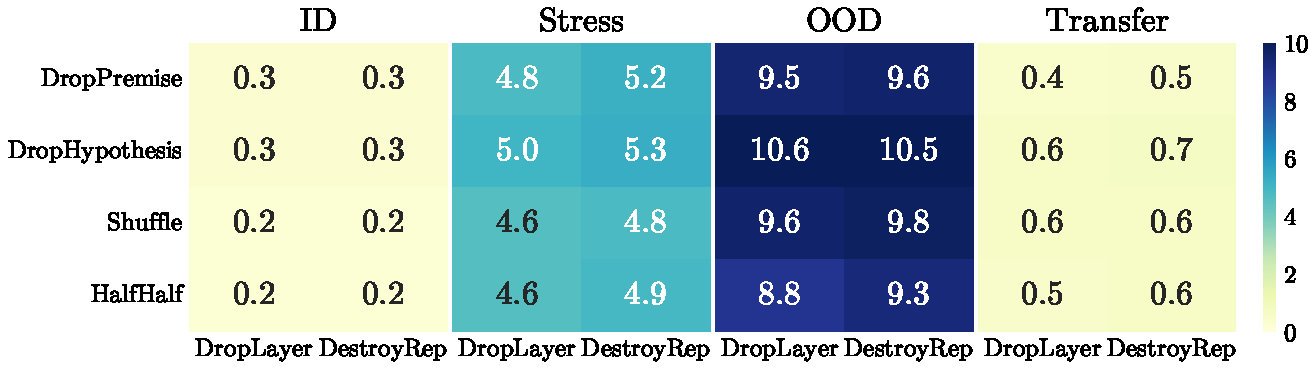
\includegraphics[width=0.5\textwidth]{figure/two_aug.pdf}
    \vspace{-20pt}    
    \caption{Debiasing performance with different combinations of explicit and implicit perturbations. 
    % In this experiment, our model employs one of the explicit perturbations and one of the implicit perturbations. 
    The values indicate relative accuracy % performance
    increase compared to vanilla fine-tuning.}
    % \vspace{-10pt}
    \label{fig:two_aug}
\end{figure}





\paragraph{Debiased Models Are Still Biased}
Our results in Table~\ref{tab:main} and prior reports~\citep{mendelson-belinkov-2021-debiasing,ravichander-etal-2023-bias} show that debiased methods can still be biased. For example, \MASK and \KW show higher levels of biases than \FT
% (without any debiasing objective) 
by 3.7 and 4.2 points on the stress test set~\citep{naik-etal-2018-stress} respectively. These results emphasize the need for modeling multiple types of biases, and highlights the advantages of our approach.
% Similar results have been reported in previous works~\citep{mendelson-belinkov-2021-debiasing,ravichander-etal-2023-bias}.

\paragraph{\OursCL Maintains Generalization across Biases}
Bias in existing methods may be because of their tendency to over-specialize in specific types of biases. \textbf{Table~\ref{tab:subset}} summarizes the performance of debiasing models across different subsets of the stress set. \OursCL achieves the maximum average performance with smaller standard deviation across these subsets, indicating that it does not overfit to specific biases. We attribute such resilience to \OursCL's incorporation of both explicit and implicit perturbations, along with the randomness in implicit perturbations, which allows the model to effectively handle diverse set of biases.

% \begin{table}
% \centering
% \setlength{\tabcolsep}{3.9pt}
% \renewcommand{\arraystretch}{0.9}
% \begin{tabular}{l|c}
% \hline
%     Model & Val. \\
%     \hline
%     Vanilla    & 78.9 \\
%     \MASK      & 70.2 \\
%     \KW        & 73.8 \\
%     \ETEPoe    & 67.4 \\
%     \RUBI      & 69.5 \\
%     \hline    
%     \OursCL    & 54.9 \\
%     \hline
%   \end{tabular}
% \caption{Performance on in-domain validation set of MNLI when feeding shuffled input.}
% \label{tab:un-lang}
% \end{table}


% \subsection{Identify spurious data}
% How to use our model to identify spurious data points in the dataset.

% 1) Look at the output of bias branches

% 2) Look at the attention weights


\begin{table}
\footnotesize
\centering
% \setlength{\tabcolsep}{3.9pt}
% \renewcommand{\arraystretch}{0.9} 
\begin{tabular}{l|lc}
\toprule
\textbf{Model} & \textbf{Param} & \textbf{Time (hr)} \\
\midrule
    \textbf{\FT}   & 110M + 2K & 4.2 \\
    \midrule
    \textbf{\MASK} & + 28M + 2K & 5.3 \\
    \textbf{\KW}   & + 3K & 6.3 \\
    % weak learner & 4.1 \\ 
    \textbf{\ETE}  & + 30K & 5.5 \\
    \textbf{\IE}   & + 50 $\times$ 2K & 7.2 \\
    \textbf{\READ} & + 28M + 2K & 4.9 \\
    \midrule
    \textbf{\OursCL} & + 2 $\times$ 2K & 4.9 \\
    \bottomrule
  \end{tabular}
  \caption{Efficiency of debiasing models on MNLI.}
  \vspace{-20pt}
  \label{tab:eff}
\end{table}

\paragraph{Efficiency}
We evaluate the efficiency of different debiasing methods in terms of number of trainable parameters and training time. 
As \textbf{Table~\ref{tab:eff}} shows,  \OursCL introduces only 4K additional parameters, which is significantly less than 100K in \IE with 50 classifiers, and 28M in \MASK and \READ with an extra weak model. This highlights the efficiency gains from the proposed perturbation operations. Furthermore, \OursCL has the shortest training time. \OursCL achieves these efficiencies without requiring additional training data, operating only by generating diverse views of the input data.


% \subsection{Discussion}\label{sec:discusion}
\paragraph{Perturbation for Data Augmentation}
The explicit perturbation operators proposed in our framework offer a valuable opportunity for data augmentation, leading to improved performances on existing debiasing methods (See Table~\ref{tab:res_aug} in Appendix).


\paragraph{Bias in Different Parts of Inputs}
In our experiments with single explicit perturbations, we find that DropPremise and DropHypothesis lead to similar performances on MNLI, 
% Table~\ref{tab:bias_type} in Appendix~\ref{sec:detail_type_of_bias}, 
showing that there exists dataset bias in premise, potentially as much as those in hypothesis. However, many existing methods tend to overlook biases in the premise in NLI datasets.
%
In addition, biases can often emerge from the interplay of various parts of inputs, rather than a single source. HalfHalf and Shuffle perturbations can capture such types of biases by perturbing the entire inputs. We note that while additional weak learners can potentially capture biases from multiple sources~\citep{utama-etal-2020-towards,sanh2020learning,meissner-etal-2022-debiasing}, their effectiveness  is likely limited by the capabilities of the weak models. 
Our approach addresses dataset biases through a multiview approach to bias, which leads to a more robust debiasing process.






% \paragraph{Connection to other methods} Several existing debiasing methods can be viewed as special cases of the proposed framework. The approaches presented in~\cite{karimi-mahabadi-etal-2020-end,clark-etal-2019-dont,sanh2020learning} can be seen as applying our explicit perturbation DropPremise and employing PoE as the fusion technique. Similarly, the approaches described in~\citep{ghaddar-etal-2021-end,sanh2020learning,meissner-etal-2022-debiasing} align with the application of our implicit perturbation ``DropLayer'' and the use of PoE as the fusion technique. In addition, the approach in~\citep{utama-etal-2020-towards}, which employs an under-trained model as a weak learner, can be seen as the implicit perturbation DestroyRep within our framework.
%
% Finally, compared to debiasing contrastive learning (DCT)~\citep{lyu2023featurelevel}, the normal distribution across classes serves as the positive example for biased inputs and negative example for intact input in our framework.

% \paragraph{Broad applicability of our framework}
% Our framework can be applied to a broad range of tasks. 
% Both the perturbations and the contrastive objective are task-agnostic, making our method applicable to various NLP tasks. For example, in case of single sentences in tasks like sentiment analysis, our method can be leveraged by implementing $\mathcal{P}_{Sub}$, which involves dropping part of the input sentence. This flexibility set our framework apart from existing debiasing methods, which often lack such adaptability or may be confined to specific model architectures. 
% %
% In addition, our framework is not limited to Transformer-based models. For example, debiasing mask~\cite{meissner-etal-2022-debiasing} prunes model parameters except those pertaining to embedding and classifier layer. Our framework is not constrained by this restriction. This means that it can be applied to various tasks, including knowledge graph embedding in which trainable parameters contain only embeddings, such as TransE~\citep{NIPS2013_1cecc7a7}, in which relationships between entities is interpreted as translations operating on the low-dimensional embeddings of the entities.

% as they are mainly designed to debias NLI tasks. \citet{karimi-mahabadi-etal-2020-end,clark-etal-2019-dont} are restricted by the bias in the hypothesis part in sentence-pair tasks.
%

